\chapter{Background}

\section{CERN}

The European Organization for Nuclear Research is a research organization that operates the world’s largest and most powerful particle accelerator, the Large Hadron Collider.

At CERN, 2500 staff members design, construct and operate the research infrastructure, in addition to more than 17500 users and scientists of 110 nationalities, from institutes in more than 70 countries.

The LHC collides two beams (\textit{bunches}) of protons at a combined energy of 13 TeV, accelerating them around a 27 km ring of superconducting magnets until they reach 99,9999990 \% of the speed of light.


Exploiting these collisions is the responsibility of large international scientific \textit{collaborations}. Each experiment, guided by a collaboration, has a detector, a large experimental apparatus placed at a collision point.

The main collision points, shown in figure \ref{fig:cern_complex}, equipped with detectors are:

TODO

\begin{enumerate}
	\item ATLAS
	\item LHCb
	\item ALICE
	\item CMS (figure \ref{fig:cms})
\end{enumerate}

\begin{figure}
	\centerline{
		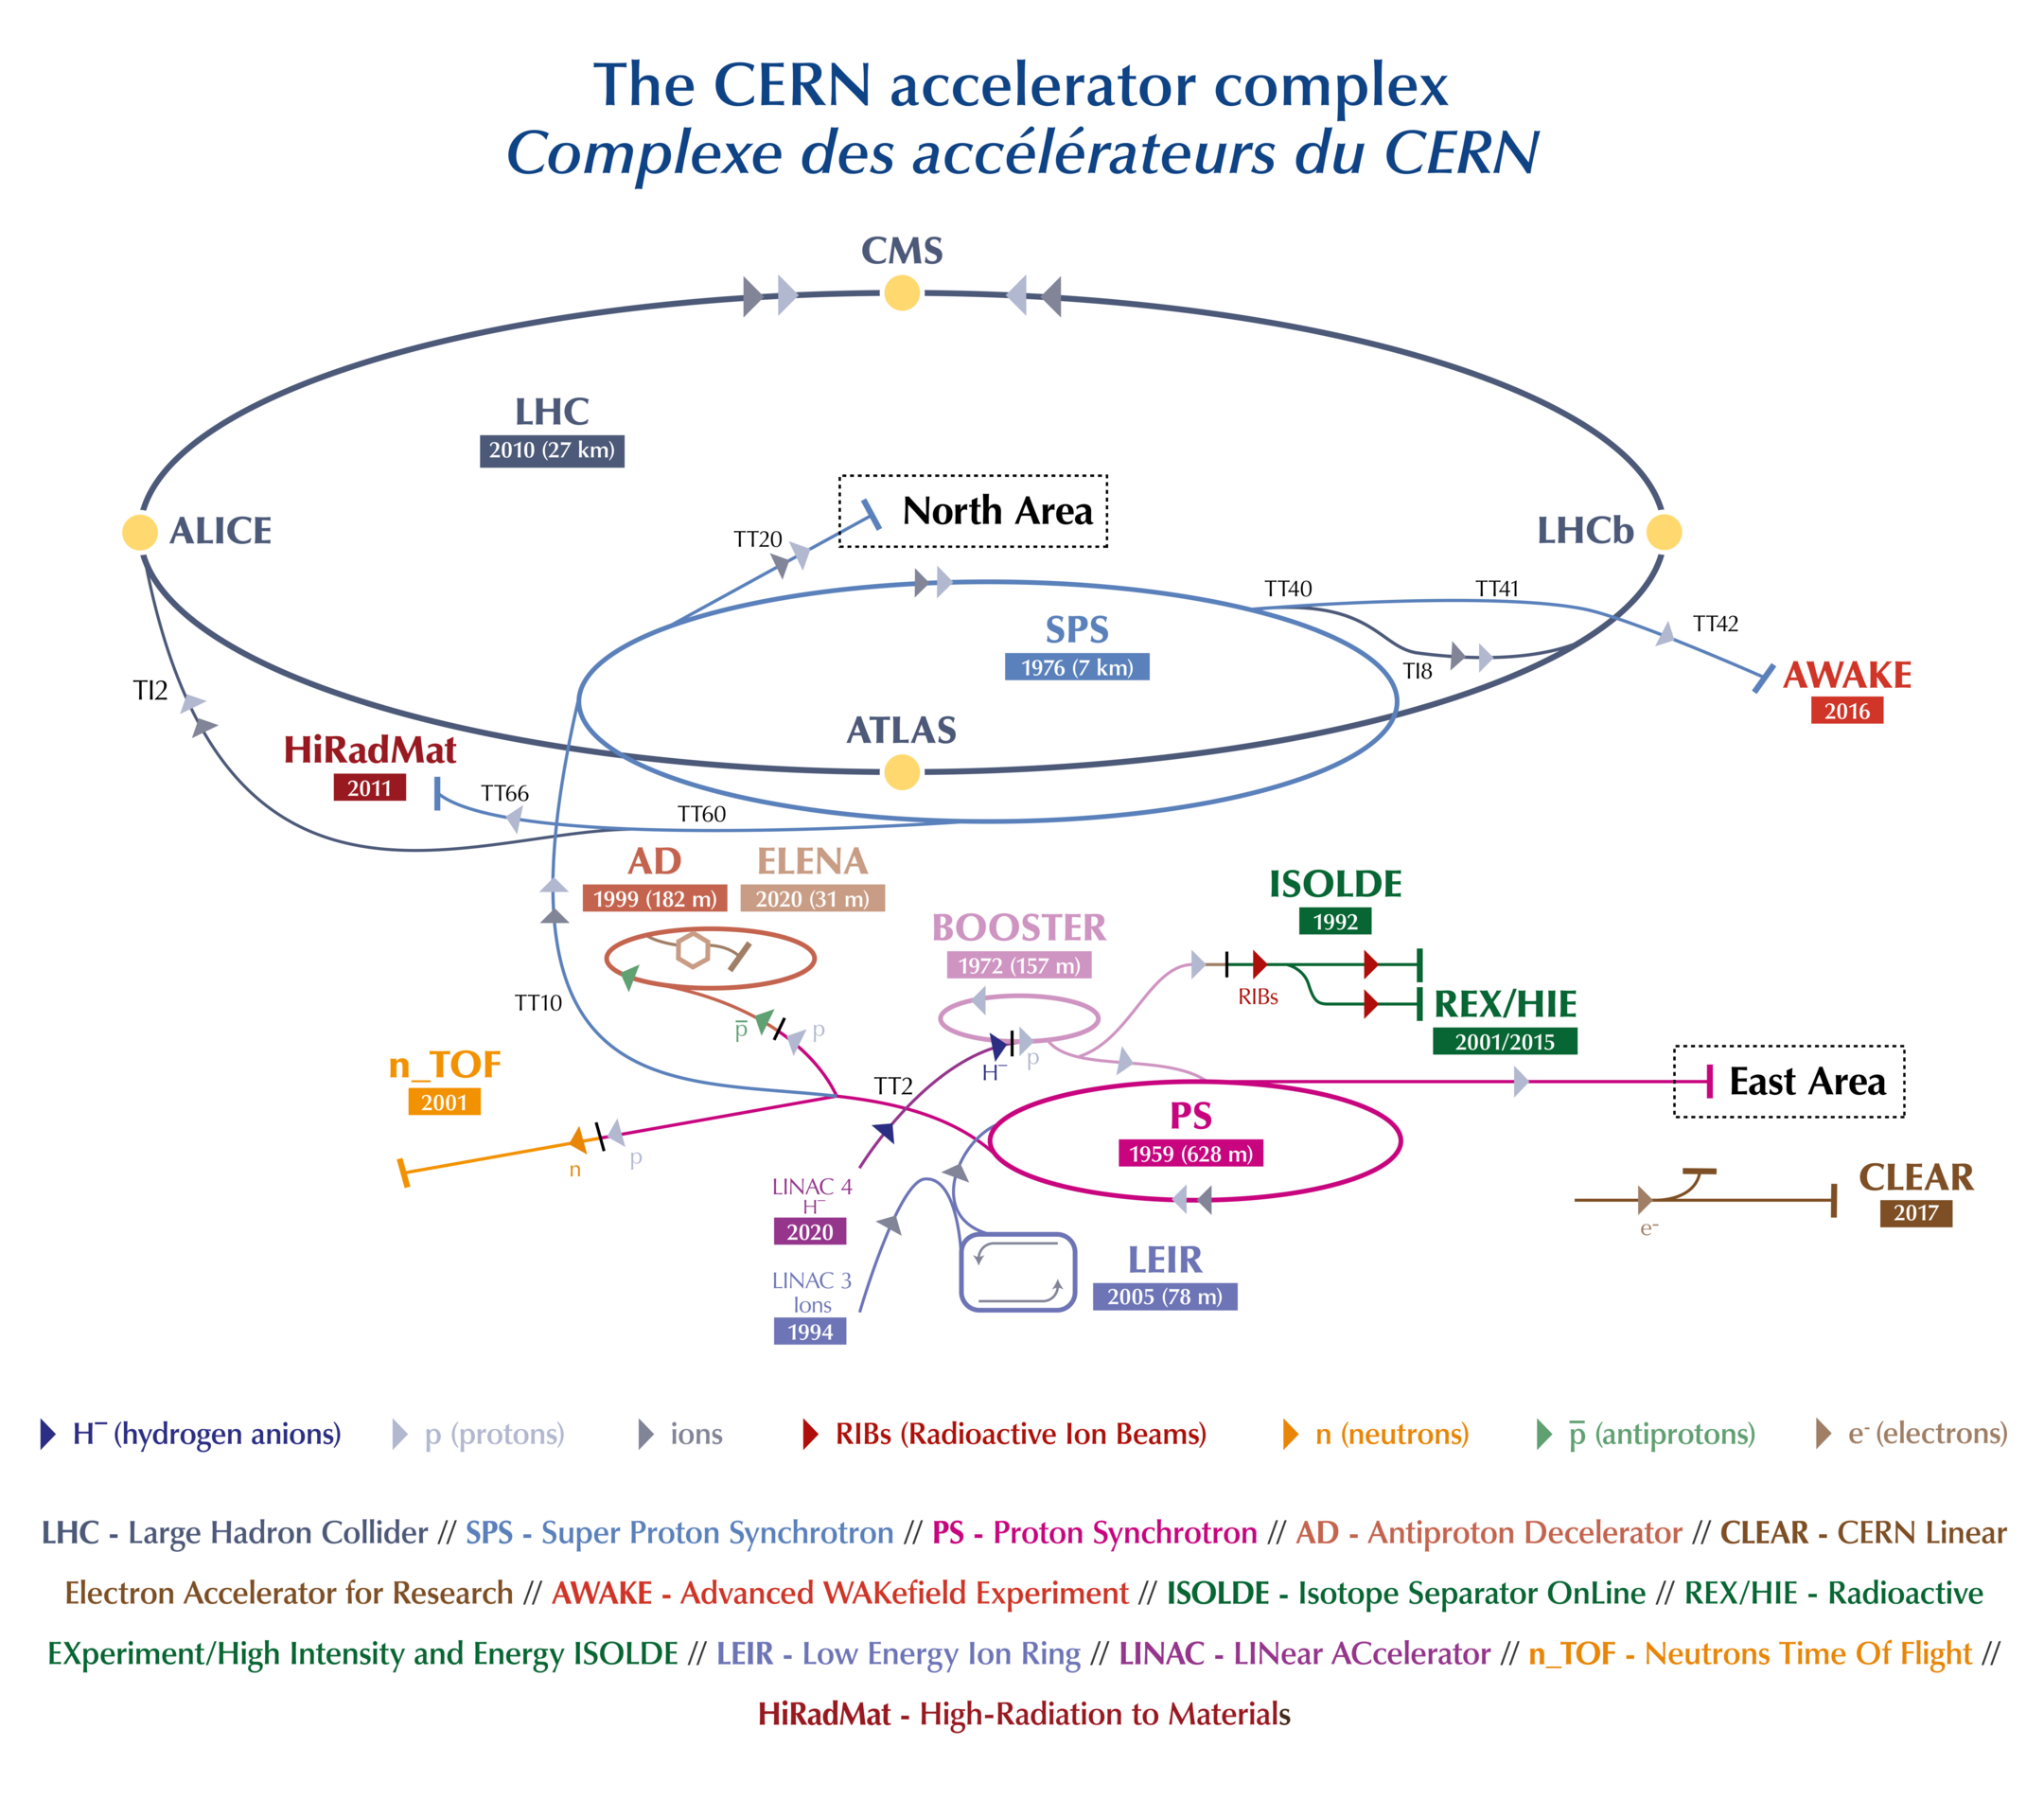
\includegraphics[width=0.75\paperwidth]{CCC-2019}}
	\caption{CERN Accelerators complex \cite{Mobs:2684277}}
	\label{fig:cern_complex}
\end{figure}

\begin{figure}
	\centerline{
		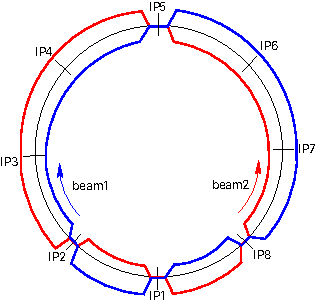
\includegraphics[width=0.4\paperwidth]{ip_1601_05235}}
	\caption{Schematic layout of the LHC collision points and beams \cite{Herr:1982430}}
	\label{fig:ip}
\end{figure}



\subsection{Computer Science}
TODO

\section{Statistics in Physics}

Many problems in physics are described or can be approximated by a small group of probability distributions. We will briefly describe them, focusing on important features exploited by Physics and Particle Physics \cite{leo2012techniques}.

\subsection{Systematic and Random Errors}

Any kind of measurement is subject to two main types of uncertainties:

\begin{enumerate}
	\item \textit{Systematic Errors} are consistent uncertainties in the bias of the data, usually associated with the measurement equipment.
	\item \textit{Random Errors} may arise from instrumental imprecision and from the inherent statistical nature of the observed class of events. Many processes in Physics are governed by the probabilistic laws of quantum mechanics, so that the number of events in a given time period is a random variable. Errors caused by the measurement of random processed are called \textit{statistical errors}. Differing values caused by many small factors not controlled by the experimenter are called \textit{instrumental errors}.
\end{enumerate}

While Systematic Errors are generally harder to handle, uncertainties caused by Random Errors follow known distributions (like a Poisson rate) or are empirically determined. As we'll see in \ref{distributions1}, repeating measurements provides larger samples to estimate these uncertanties and get more accurate data.


\subsection{Binomial}

When a problem involve repeated, independent trials with two possible outcomes, the probability is given by the binomial distribution:

\begin{equation}
	P(r)= \frac{N! }{ r! \left( N-r \right)! } p^r (1-p)^{N-r}
\end{equation}

where $p$ is the probability of success in a single trial.

% TODO: Define r and N, too
% Introduce the notions of Mean and Variance

Mean:

\begin{equation}
	\mu = \sum_{r}rP(r) = Np
\end{equation}

Variance:

\begin{equation}
	\sigma^2=\sum_r(r-\mu)^2P(r) = Np(1-p)
\end{equation}

For many practical calculations \cite{leo2012techniques}, using a Gaussian (\ref{eqn:gaussian}) is a good approximation of a Binomial when $N$ is greater than 30 and $p\geq0.05$ (taking into consideration that we are replacing a discrete distribution by a continuous one). When $p\leq0.05$ and the product $Np$ is finite, we can use a Poisson distribution.

\subsection{Poisson}
\label{distributions1}

When the probability is very small ($p \rightarrow 0$) and the numer of trials approaches infinity ($N \rightarrow \infty$) such that the mean $\mu = N p$ remains finite, the \textit{Poisson} distribution occurs:

% TODO: define r and P(r)

\begin{equation}
	\label{eqn:poisson}
	P\left( r \right) = \frac{{\mu^{ r } e ^{-\mu} }}{{r!}}
\end{equation}

If the mean is expressed as the mean per unit dimension ($\mu = \lambda t$) we can rewrite \ref{eqn:poisson} as:

\begin{equation}
	P\left( x \right) = \frac{(\lambda t) ^r {e^{ - \lambda t}} }{{r!}}
\end{equation}

\begin{figure}
	\centerline{
		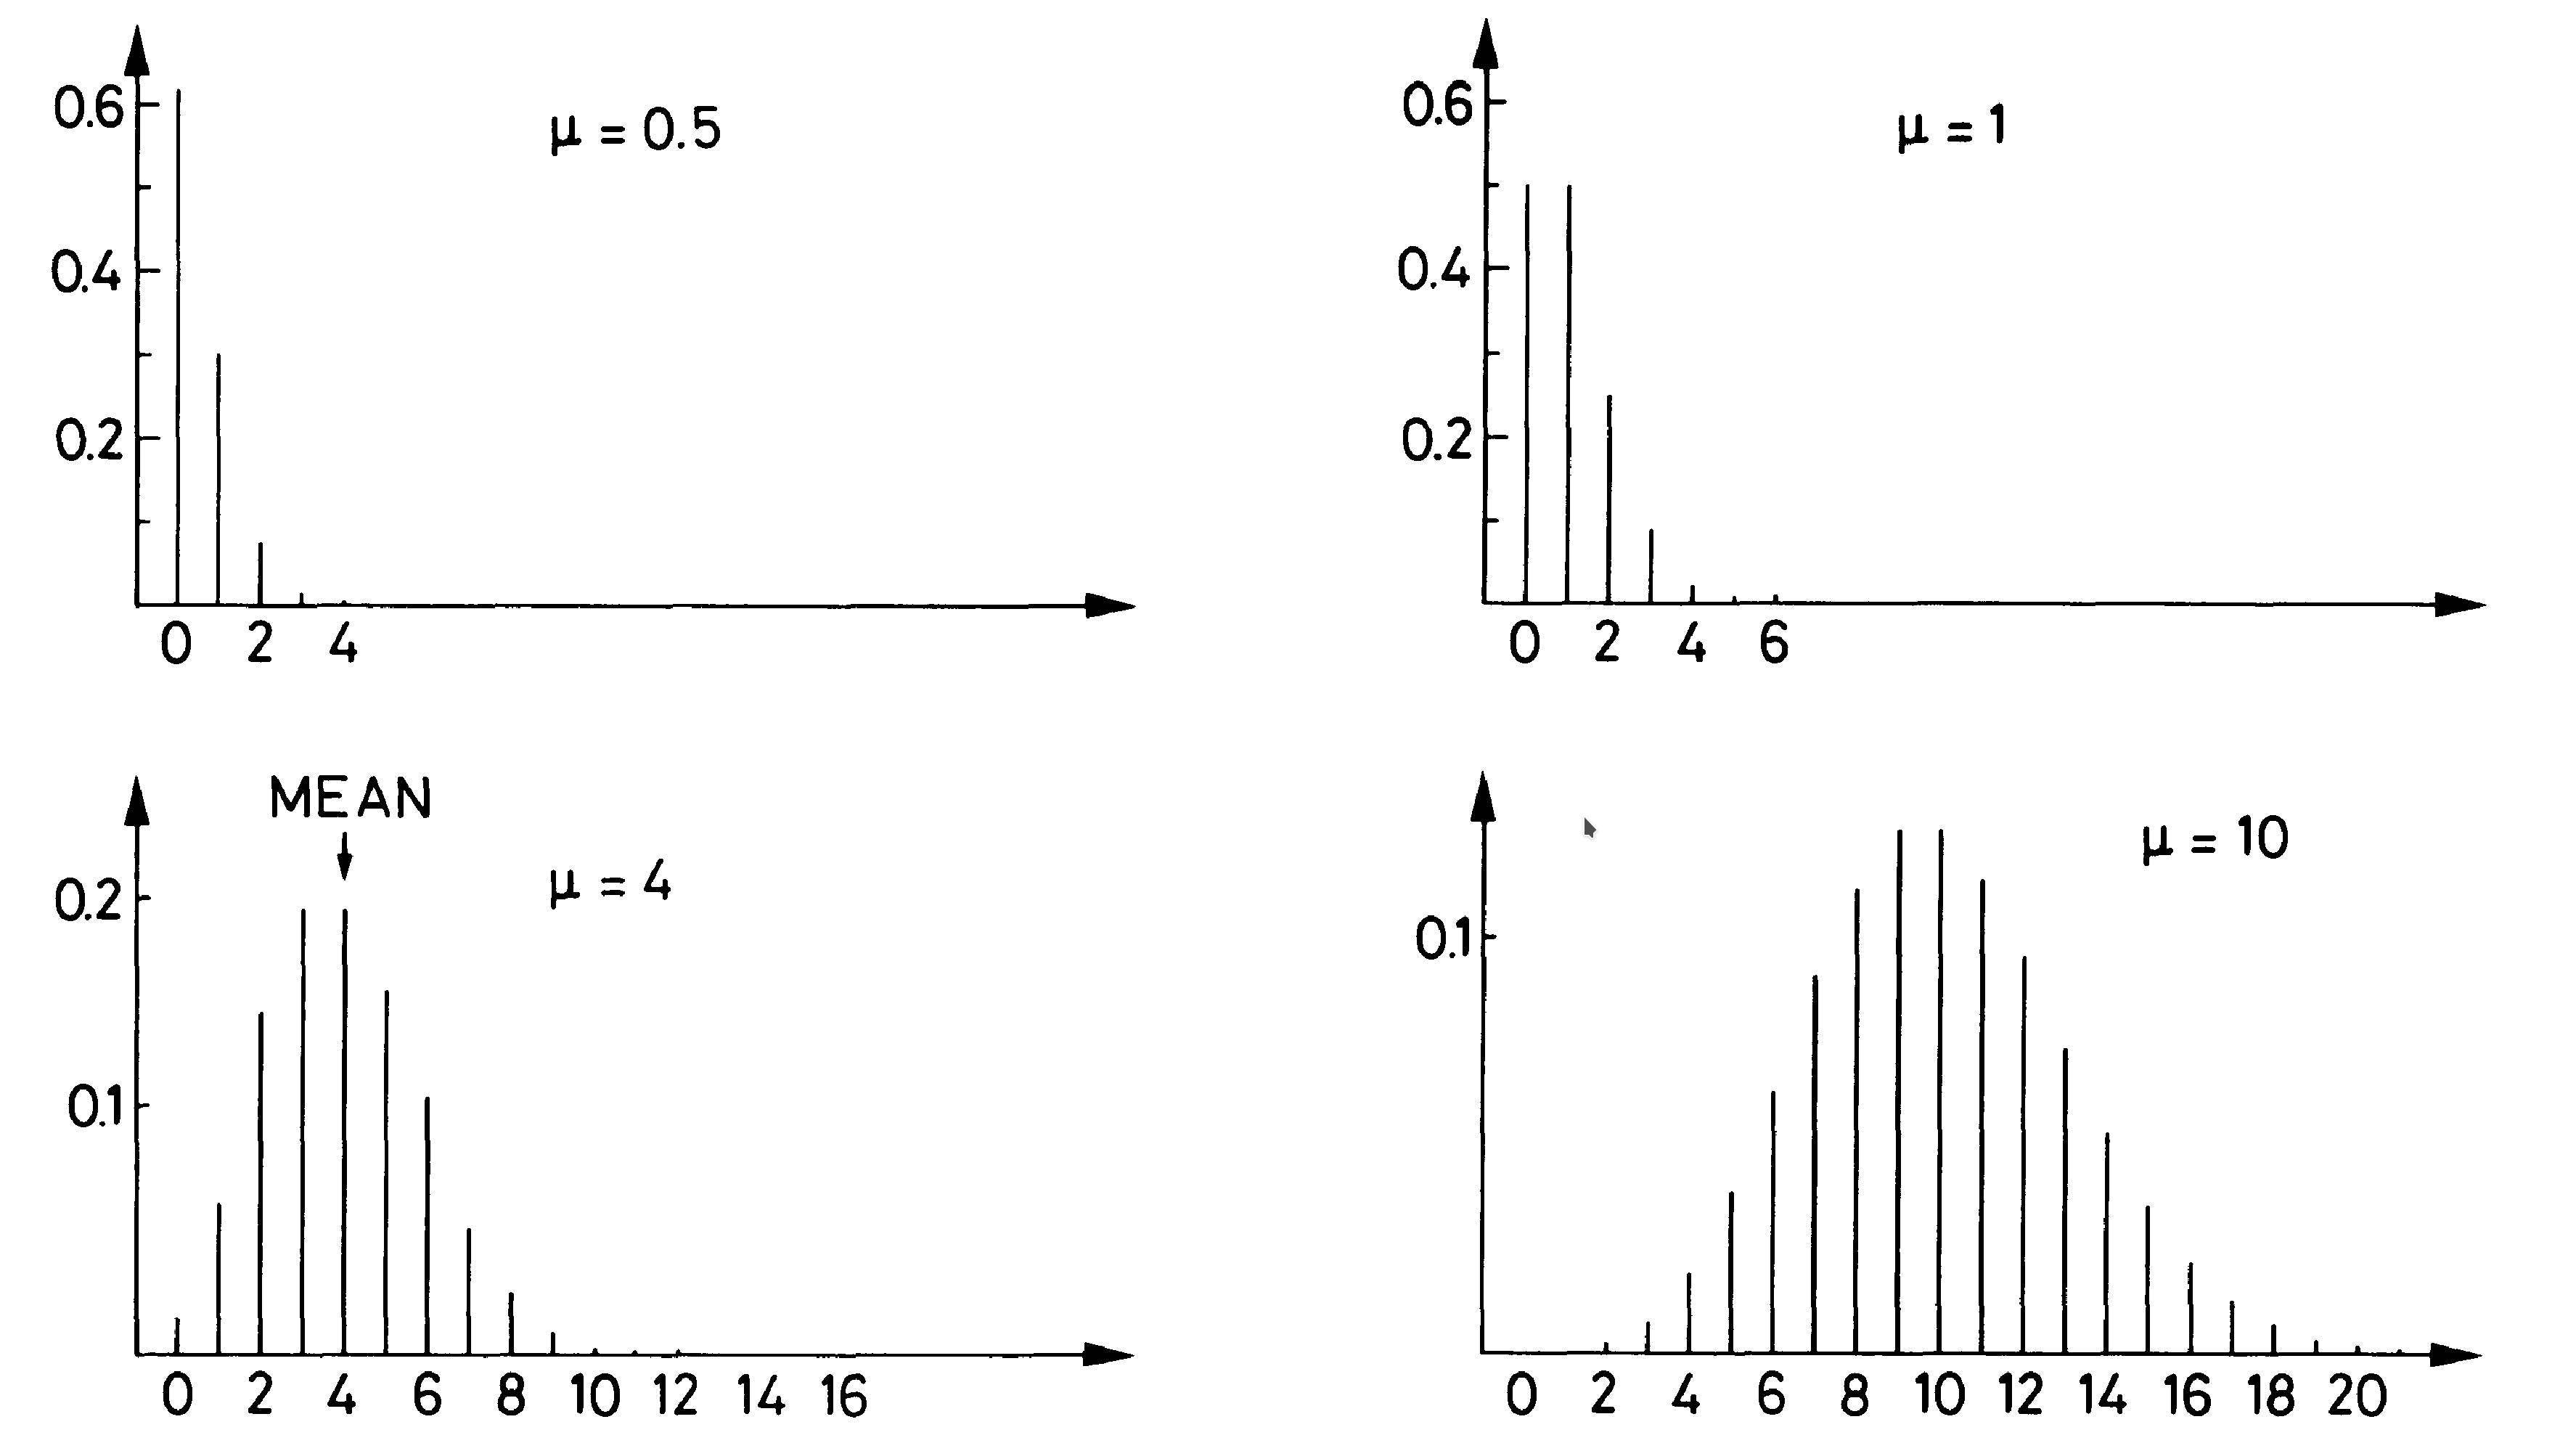
\includegraphics[width=0.5\paperwidth]{poisson}}
	\caption{Poisson distribution with various values of $\mu$ \cite{leo2012techniques}}
\end{figure}

% FIXME: The probability for a single nucleus to decay -> Probability per time unit

As an example, consider the \textit{radioactive decay} phenomena: a radioactive source such as $^{137}$Cs has a half-life of 27 years. The probability for a single nucleus to decay is $8.2 \times 10^{-10}s^{-1}$. However, even a \SI{1}{\micro\gram} contains $10^{15}$ nuclei. Since each nucleus acts as a \textit{trial}, the mean number of decay events will be $\mu = N p = 8.2 \times 10^5$, satisfying the limiting conditions. The probability of observing an event is given by \ref{eqn:poisson}.

The Poisson distribution exhibits two interesting features:

\begin{enumerate}
	\item Only mean appears, so the knowledge of $N$ and $p$ is not always required. E.g. this happens in experiments involving particle reactions where the mean counting rate is known, rather than the number of particles in the beam.

	\item This distribution only depends on one parameter: $\mu$. We can arbitrarily increase this value by repeating the experiment for higher values of $N$.
\end{enumerate}

\subsection{Gaussian}
\label{eqn:gaussian}

%TODO: Define densiti

The \textit{Gaussian} (or \textit{Normal}) is a continuos, symmetric distribution. Density is defined as

\begin{equation}
	P(x) = \frac{1}{{\sigma \sqrt {2\pi } }}e^{{{ - \left( {x - \mu } \right)^2 } \mathord{\left/ {\vphantom {{ - \left( {x - \mu } \right)^2 } {2\sigma ^2 }}} \right. \kern-\nulldelimiterspace} {2\sigma ^2 }}}
\end{equation}

Where $\mu$ is the mean and $\sigma ^2$ corresponds to the variance. The case where $\mu = 0$ and $\sigma = 1$ is called the \textit{standard} normal distribution.

\begin{equation}
	y = \frac{e^{ - \frac{{x^2 }}{2}}}{{\sqrt {2\pi } }}
\end{equation}

Any Gaussian distribution can be transformed to this reduced form trivially:

\begin{equation}
	z = \frac{x-\mu}{\sigma}.
\end{equation}

\begin{figure}
	\centerline{
		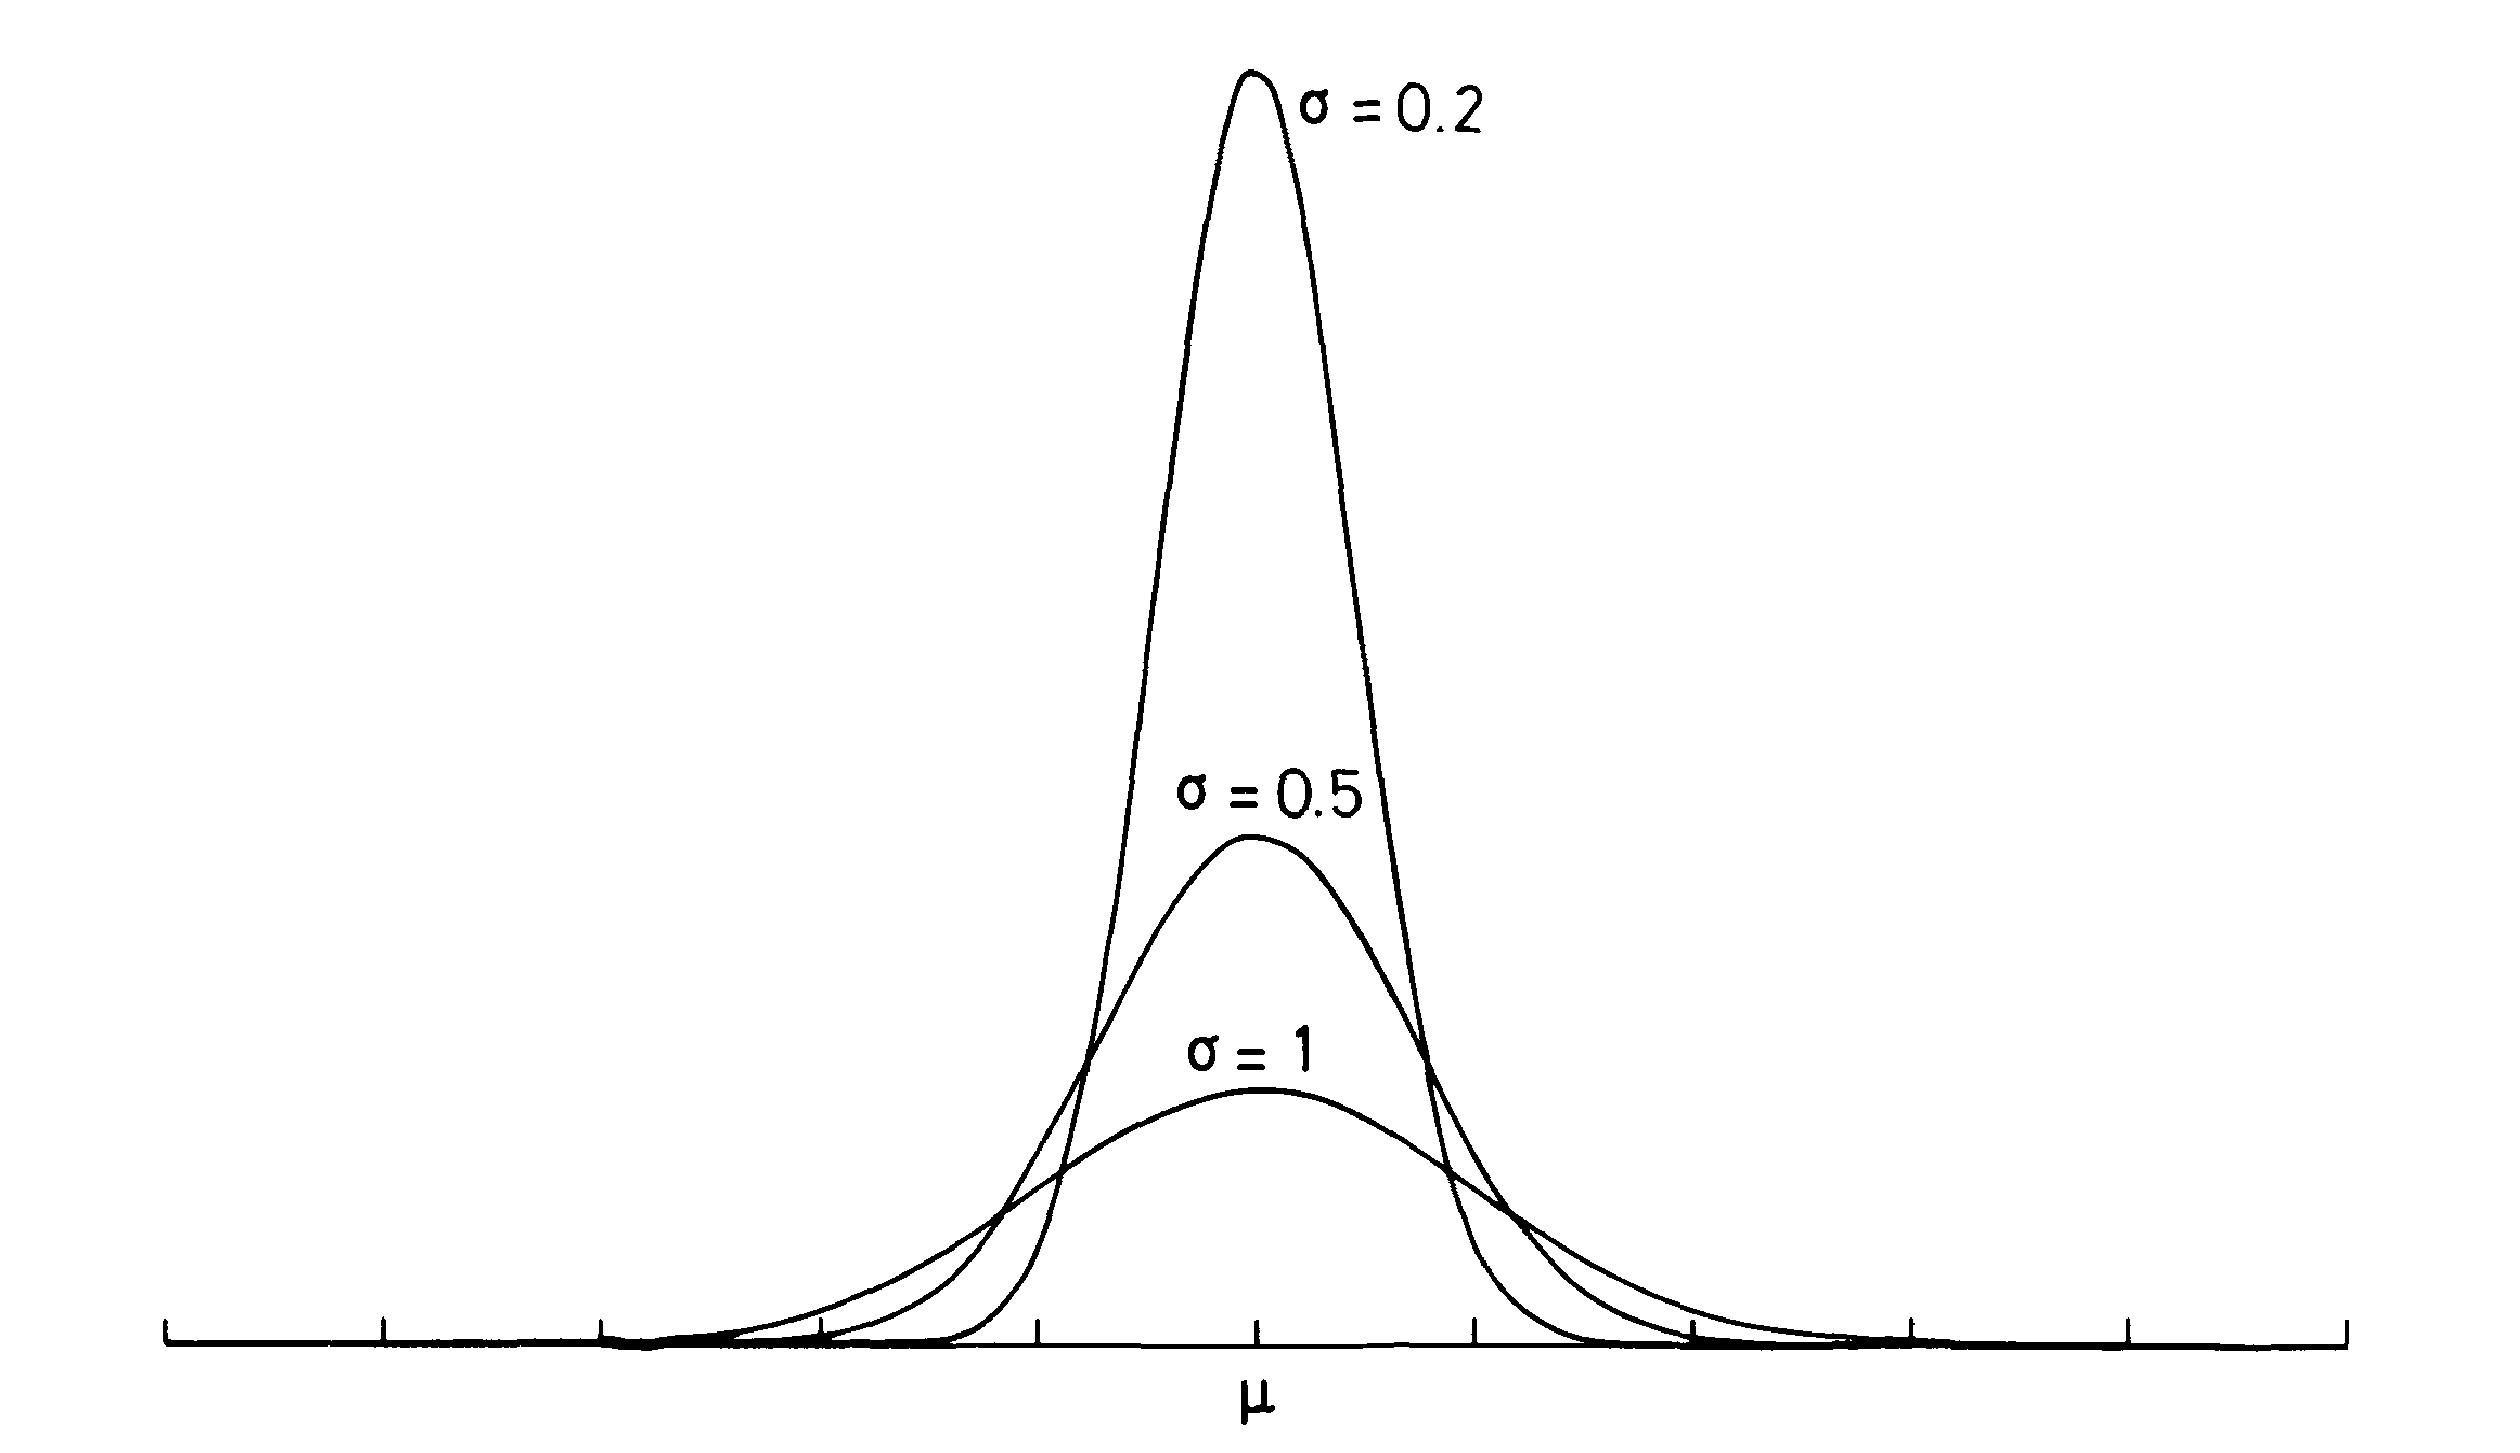
\includegraphics[width=0.5\paperwidth]{gaussian}}
	\caption{Gaussian distribution with various values of $\sigma$ \cite{leo2012techniques}}
\end{figure}

\section{Particle Physics}

Particle physics researches the nature of the fundamental parts of matter and how they interact. According to the Standard Model \cite{Quang:1998yw}, the matter is made of \textit{fermions}, classified into leptons (electrons, muons, taus and neutrinos) and quarks (up, down, charm, strange, top, bottom). Each particle have an associated antiparticle of the same mass but opposite quantum numbers.

Interactions between fermions are mediated by bosons:

\begin{enumerate}
	\item Strong interaction, mediated by gluons
	\item Weak interaction, mediated by Z and W bosons
	\item Electromagnetic interaction, mediated by photons
\end{enumerate}

Gravitational force is not taken into account. Quarks interact with all three forces, leptons are not sensitive to the strong force and neutrinos are subject only to the weak force.

Experiments are the tool to validate the current theories: the Standard Model anticipated the existence of previously undiscovered particles, such as the \textit{Higgs} Boson, observed at CERN in 2012. This particle is responsible of giving mass to the otherwise massless particles in the SM, conciliating the theory with other experimental findings (Brout-Englert-Higgs mechanism \cite{PhysRevLett.13.321, PhysRevLett.13.508}).

Current High Energy Physics research includes:
\begin{enumerate}
	\item Matter-antimatter asymmetry of the universe \cite{Bernreuther:2002uj};
	\item The not-yet discovered dark matter, which is supposed to give galaxies the extra gravity needed to explain many observed features \cite{bertone2005particle};
	\item Explanation of gravitational physics in terms of quantum mechanics (e.g. \cite{Rovelli:2011eq});
\end{enumerate}

\section{Large Hadron Collider}

%%

TODO LHC

High Energy Physics experiments need to collect a large quantity of data to attack the statistical nature of particle physics and find interesting and rare phenomena with enough accuracy.

\subsection{Cross Section}

\begin{figure}

	\centerline{
		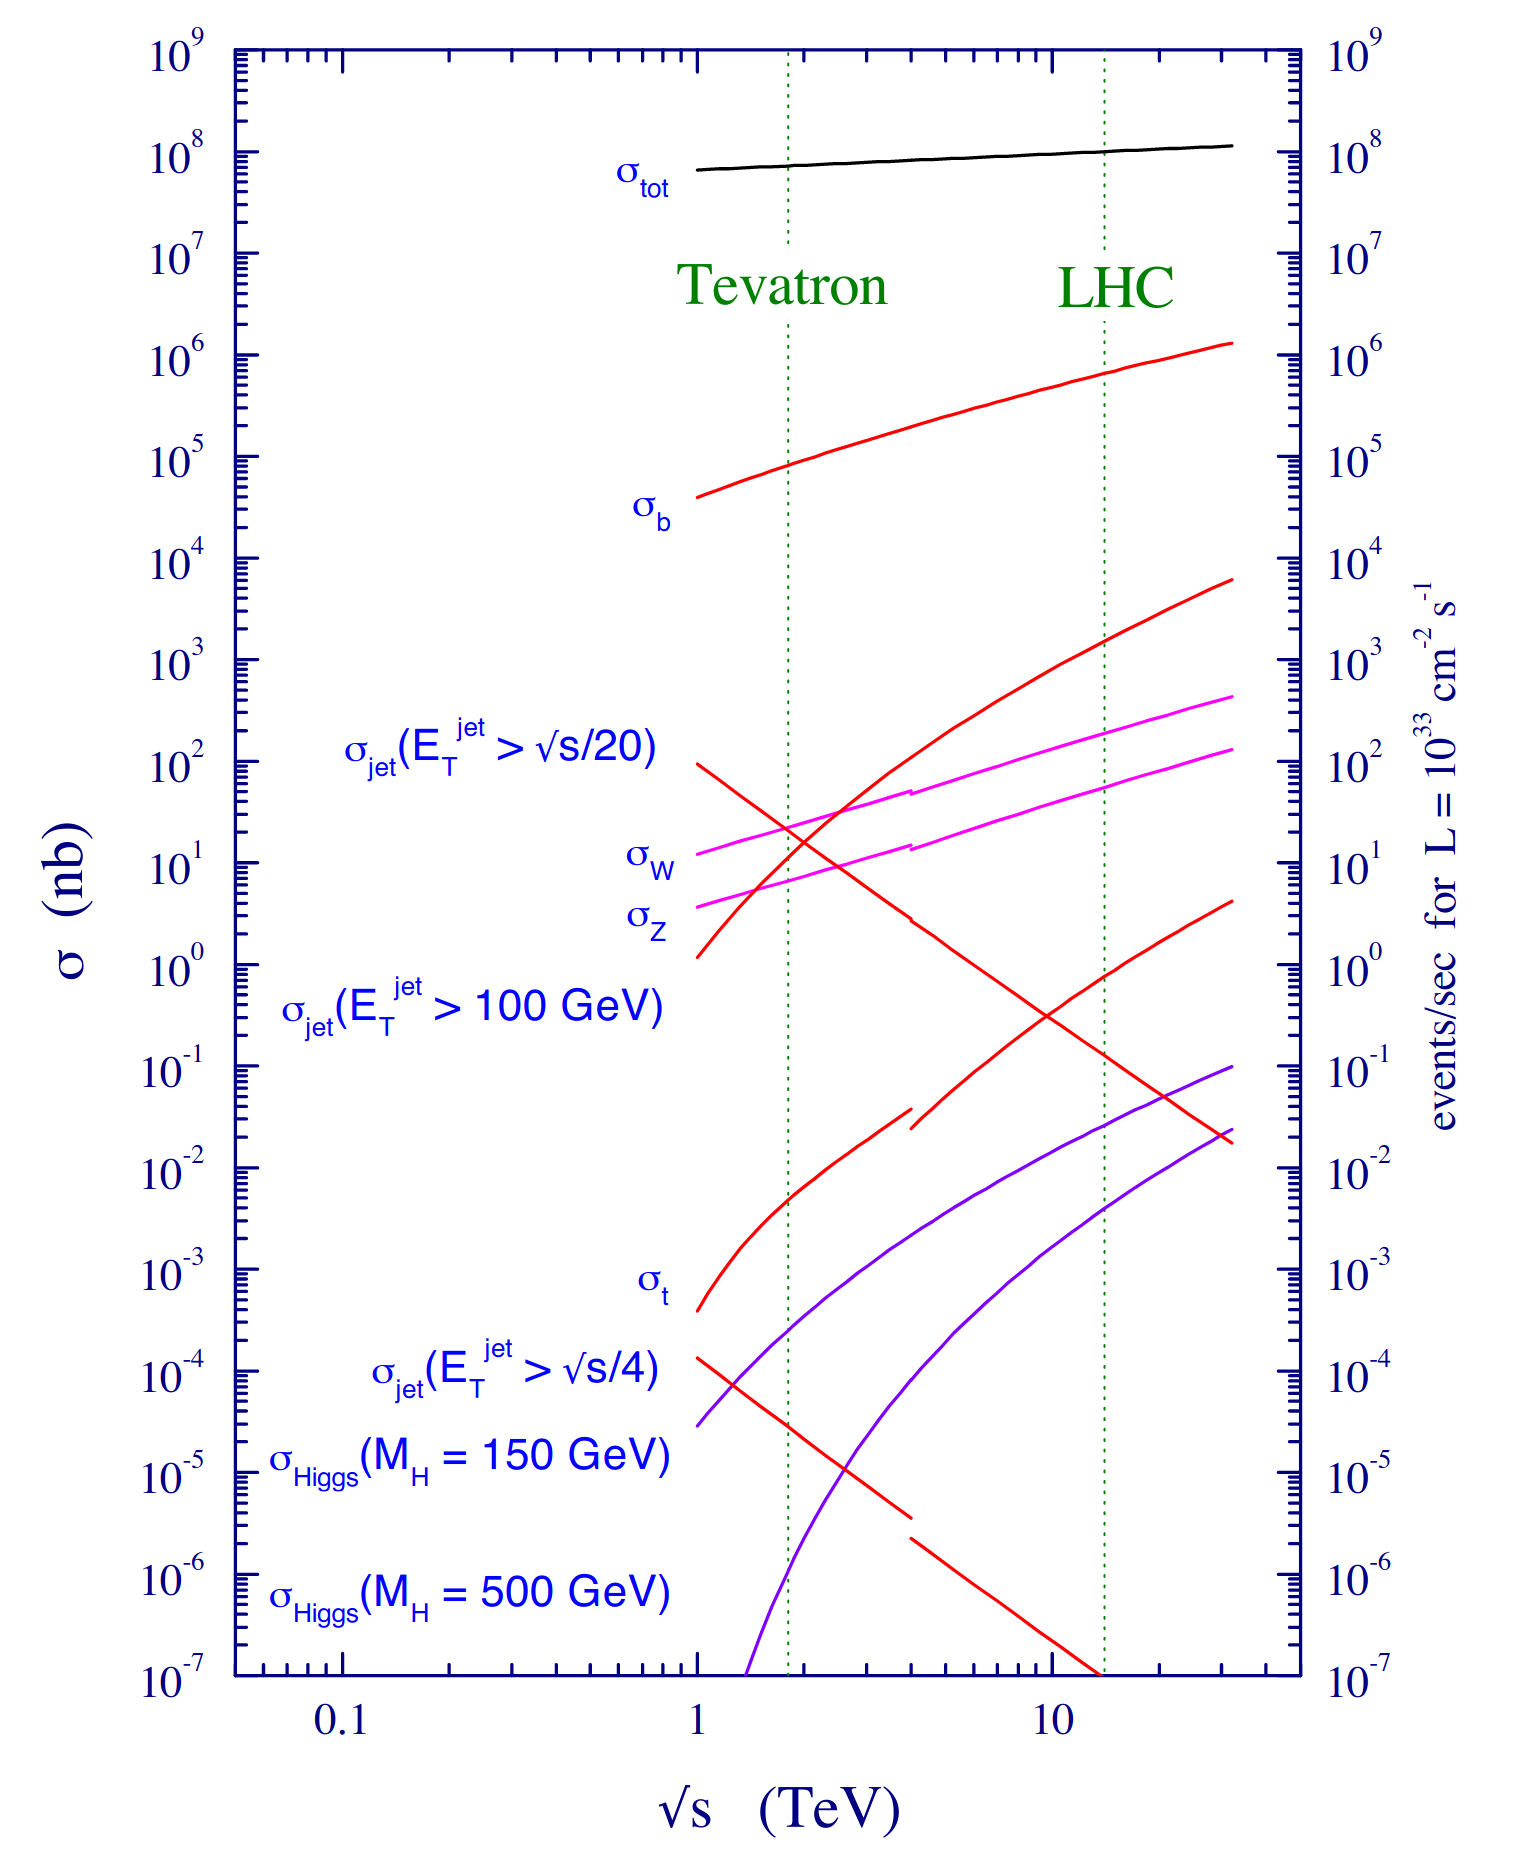
\includegraphics[width=0.5\paperwidth]{cross_sections}}
	\caption{Standard  model  cross  sections  at  the  Tevatron  and  LHC  colliders\cite{Bechtel:2009zza}}
	\label{fig:cross_sections}
\end{figure}

Cross section ($\sigma$) is one of the most important quantity in particle physics: it measures the probability that a specific process occurs in a collision of two particles. It is expressed in terms of the transverse area that the particle must hit to for that process to occur and it's measured in \textit{Barn}: $1\, b = 10^{-24} \,cm^2$.

E.g. the \textit{Rutherford cross-section} represents the probability of an alpha-particle to be deflected by a given angle during a collision with an atomic nucleus.

%TODO: Add cross section value for this example

Figure \ref{fig:cross_sections} shows $\sigma$ values for different processes. Notice how the value increments with the collision energy $\sqrt s$ (13 TeV during LHC Run 2).

\subsection{Luminosity}

This value is a measurement of the number of collisions that can potentially be produced in a point of collision per $cm^2$ and per second. It can be calculated in this way:

\begin{equation}
	L \simeq  \frac{N^2}{t S_{\text{eff}}}
\end{equation}

Where $N$ is the number of protons in each bunch, $t$ is time between bunches, $S_{\text{eff}} = 4 \pi \sigma_c^2$ is the section effective of collision.

In the LHC, $\sigma _c= 16\times 10^{-4}\, cm$, $N = 1.15\times10^{11}$, $t = 25 \times 10^{-9}\, s$, leading to a design luminosity of $10^{34}\, cm^{-2}s^{-1}$.

\subsection{Delivered Luminosity}

The actual luminosity value reached in the points of collision and recorded by the detectors is called Delivered Luminosity.

A number of factors influence this value (TO CHECK):

\begin{enumerate}
	\item Adjustments of the LHC beam-optics (emittance scan);
	\item Prescale settings;
	\item Lumi-levelling;
	\item Physiological decrease, due to the fact that protons get consumed by collisions.
\end{enumerate}

Figure \ref{fig:lum_evolution} shows the evolution of the delivered luminosity to the ATLAS, CMS and LHCb experiments.


\begin{figure}
	\centerline{
		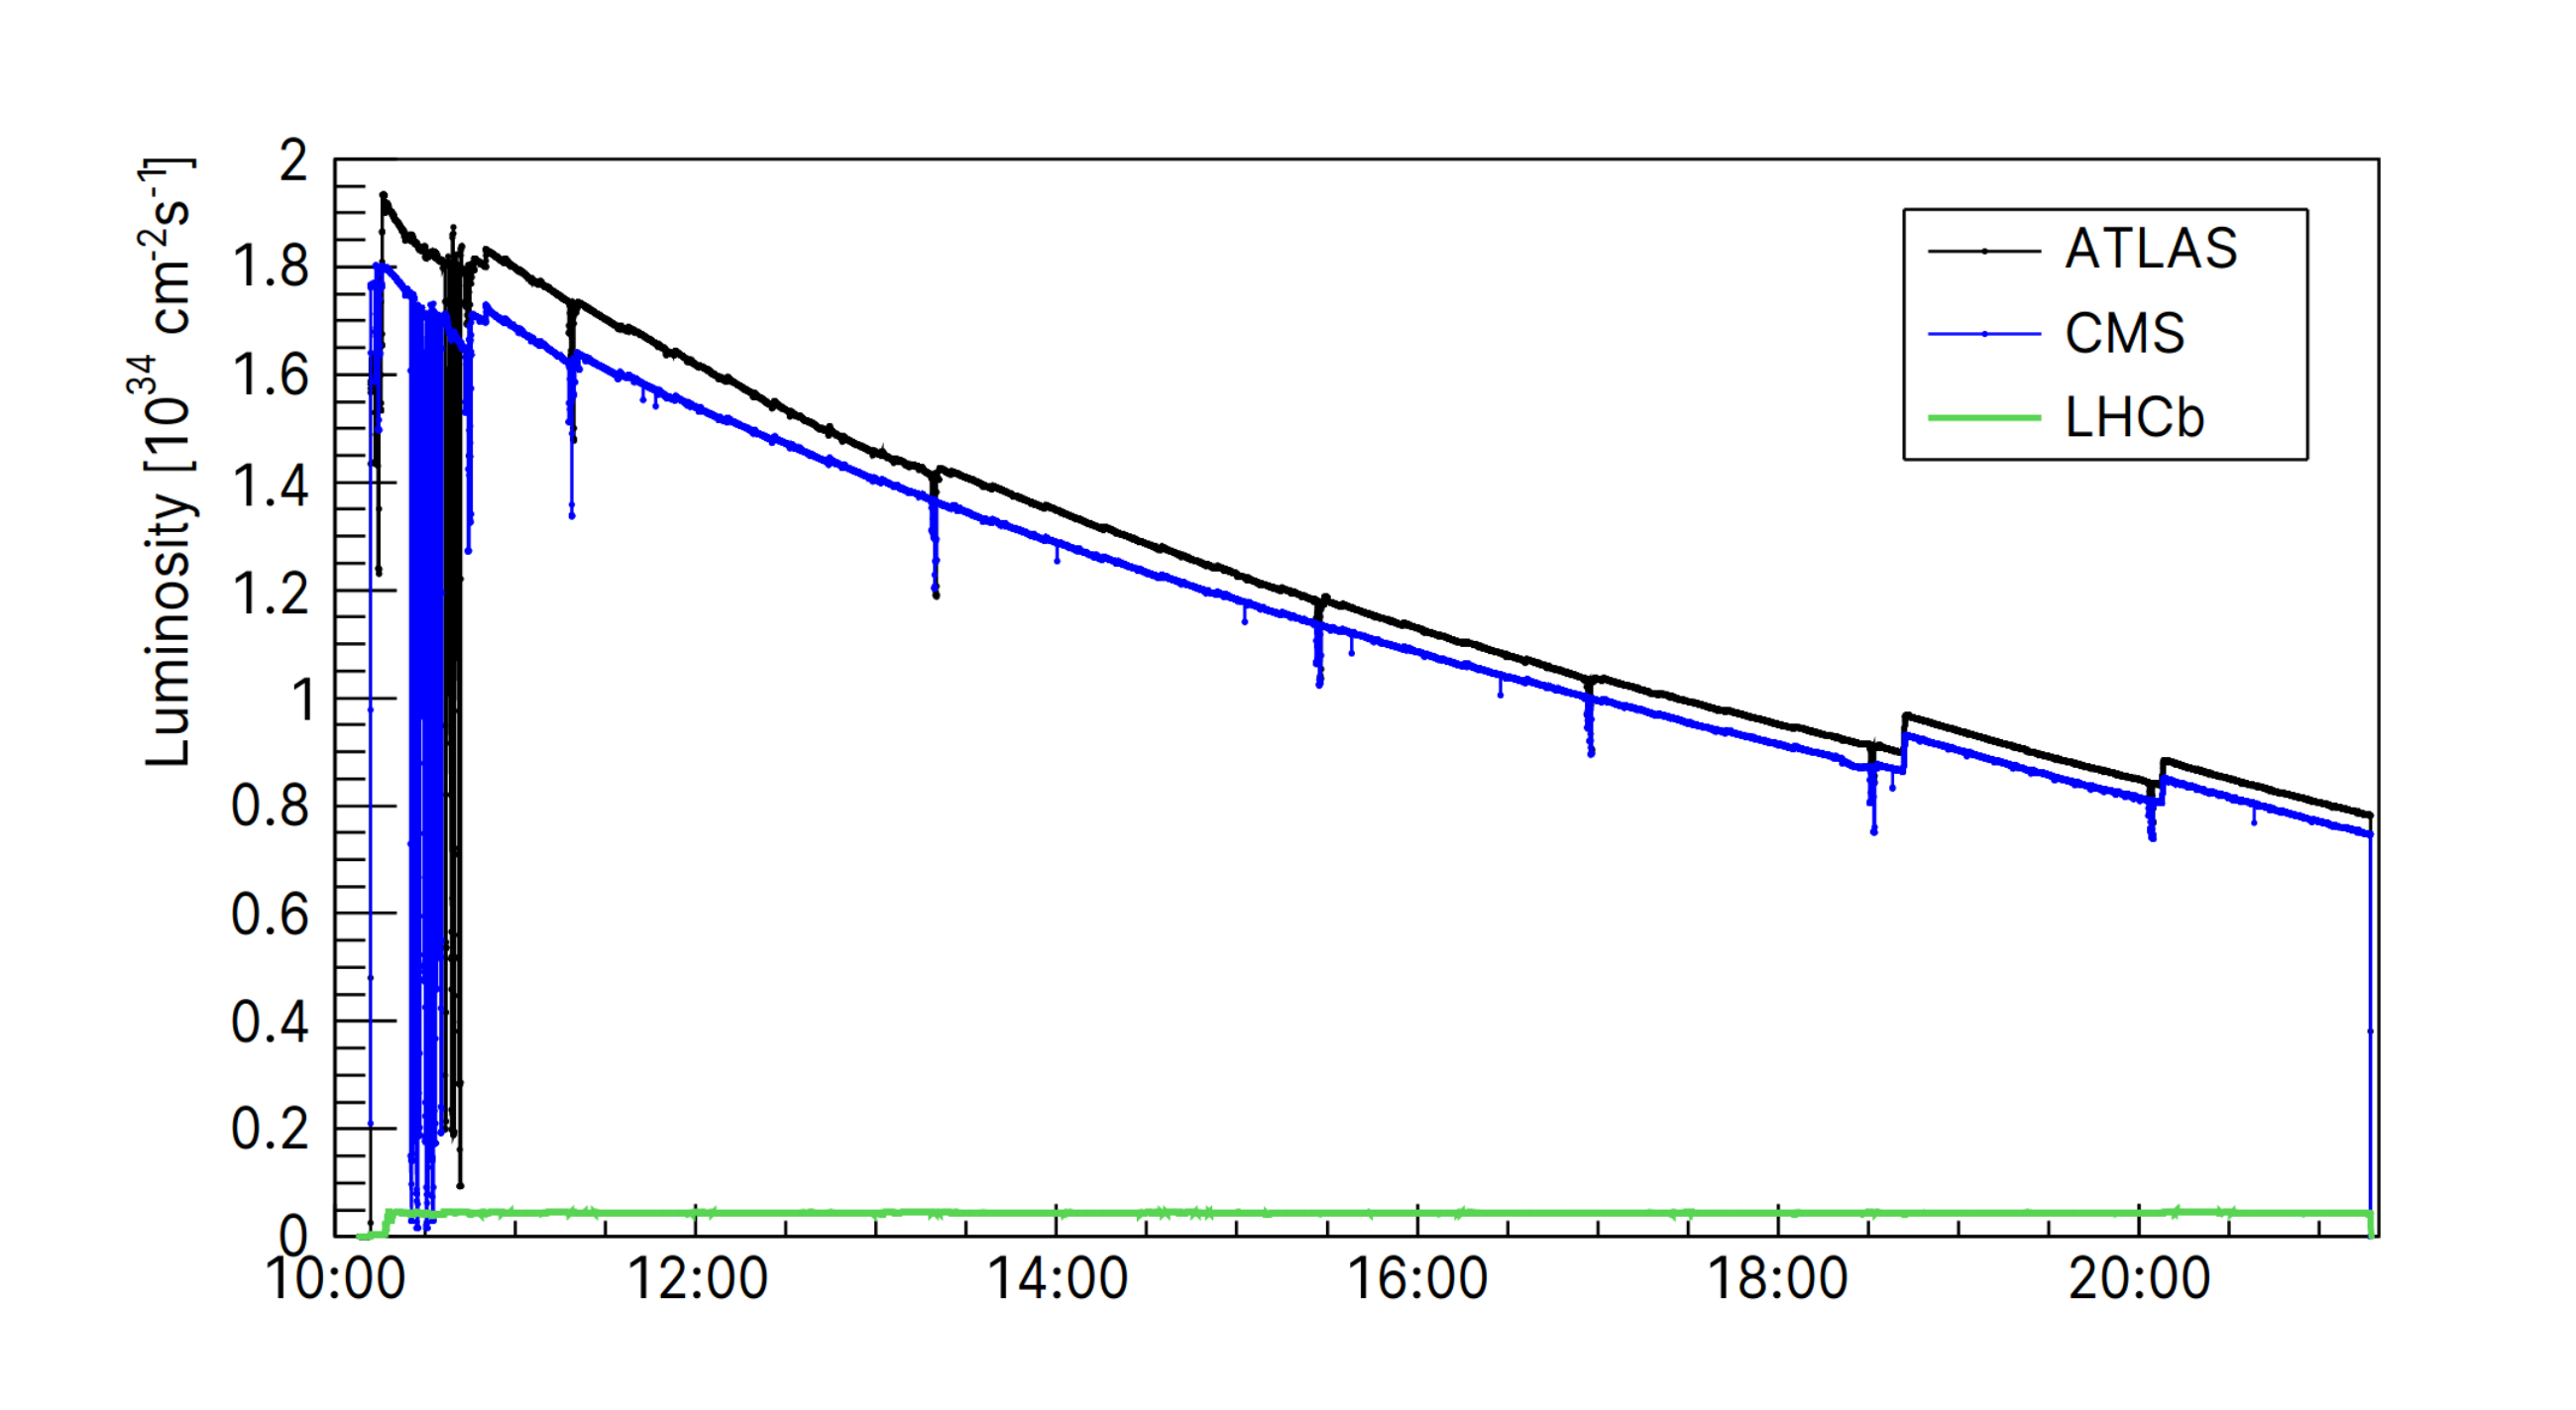
\includegraphics[width=0.5\paperwidth]{inst-lumi}}
	\caption{Example for the luminosity evolution of the ATLAS, CMS and LHCb experiments in a typical fill of the 2018 run. The luminosity of LHCb is levelled by beam separation. The upward steps of the ATLAS and CMS luminosities in the second half of the fill are due to $\beta\text{*}$ levelling
		\cite{Wenninger:2018cgs}}
	\label{fig:lum_evolution}
\end{figure}


\subsection{Integrated Luminosity}

The integral of the delivered luminosity over time is called integrated luminosity. It is a measurement of the collected data size, and it is an important value to characterize the performance of an accelerator.

\begin{equation}
	L = \int Ldt
\end{equation}

It's expressed in inverse of cross section, usually in $\text{femtobarns}^{-1}$ ("Femto" indicates a factor of $10^{-15}$ so $\text{1 femtobarn} = 1 \text{fb} = 10^{-15} \text{b} = 10^{-39} cm^2 $).

One inverse femtobarn is equal to approximately 100 trillion proton-proton collisions.

\begin{figure}
	\centerline{
		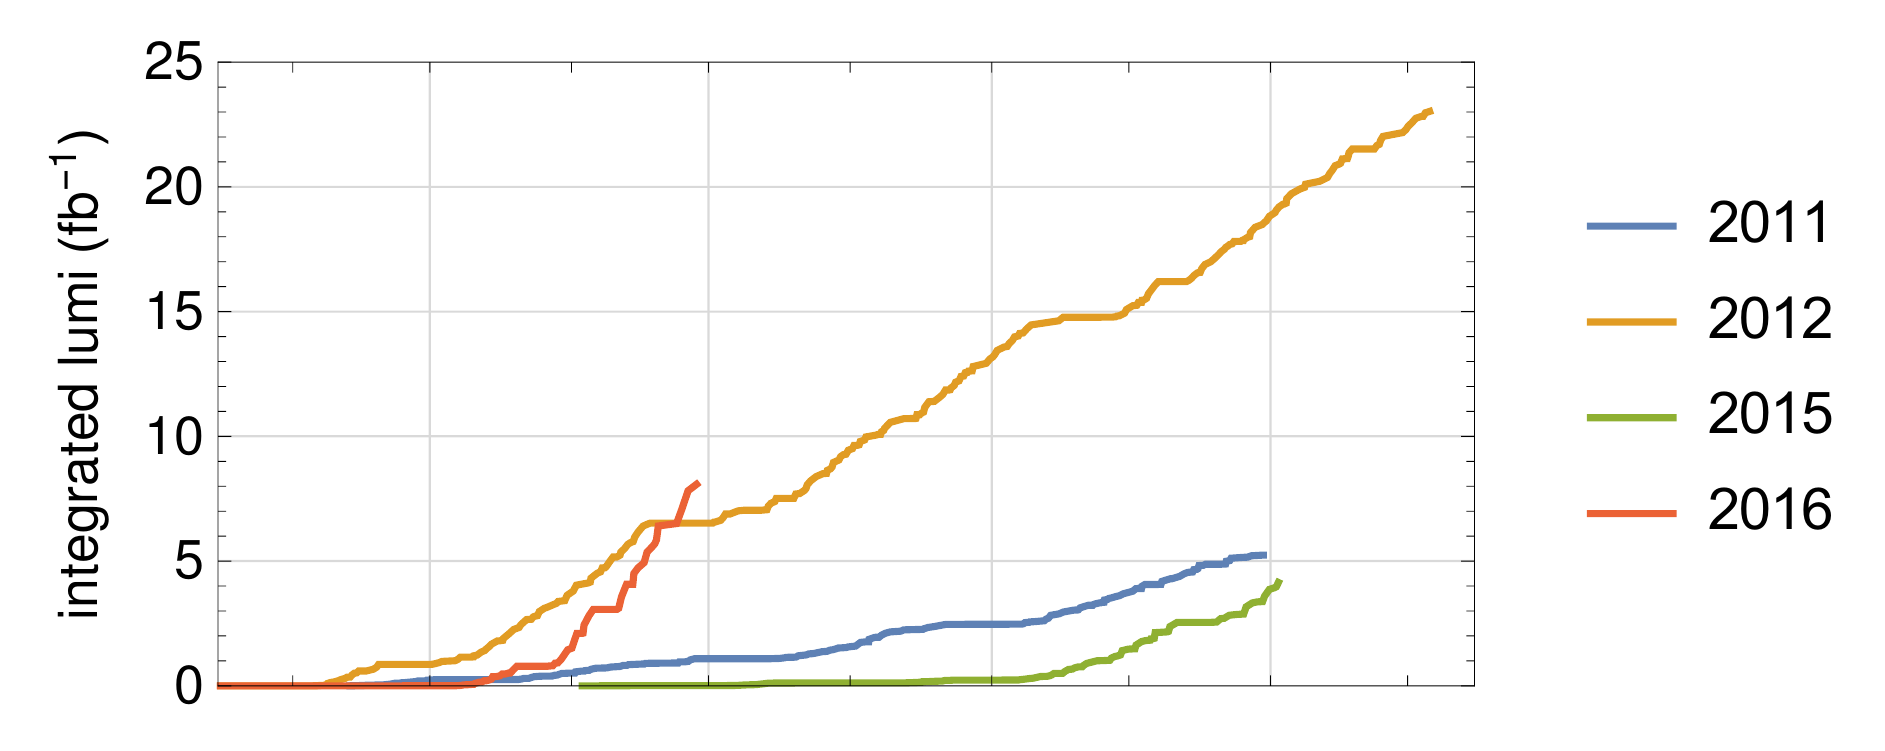
\includegraphics[width=0.5\paperwidth]{integrated_lumi_atlas}}
	\caption{Integrated luminosity at ATLAS experiment \cite{Bruce:2016iew}}
\end{figure}

\subsection{Standard Deviation and Significance}

Searches in Particle Physics are done looking for an excess above background: a discovery of a particle involves knowing the amount of background events to except and being confident that the excess is not the result of a statistical fluctuation of this background.

% TODO: qui serve che tu richiami esplicitamente il fatto che stai trattando la produzione e la selezione di eventi con una gaussiana. Io non citerei il numero di sigma ma bensi’ la probabilita’ delle code: 68%, 95% etc. etc.  Alla fine poi puoi spiegare che corrispondono ad integrare la gaussiana in intervalli di 1, 2, 3 standard deviations

The scientific process requires quantification of the probability that excesses are genuine: this is why the "number of $\sigma$" is crucial in validating discoveries: it represents the width of the Gaussian distribution, as we explained in \ref{eqn:gaussian}. The greater number of $\sigma$, the minor will be the probability that the observed excess can be explained by a background fluctuation.
At $3\sigma$ we talk about an evidence, while at $5\sigma$ we are in front of a discovery.

\begin{figure}
	\centerline{
		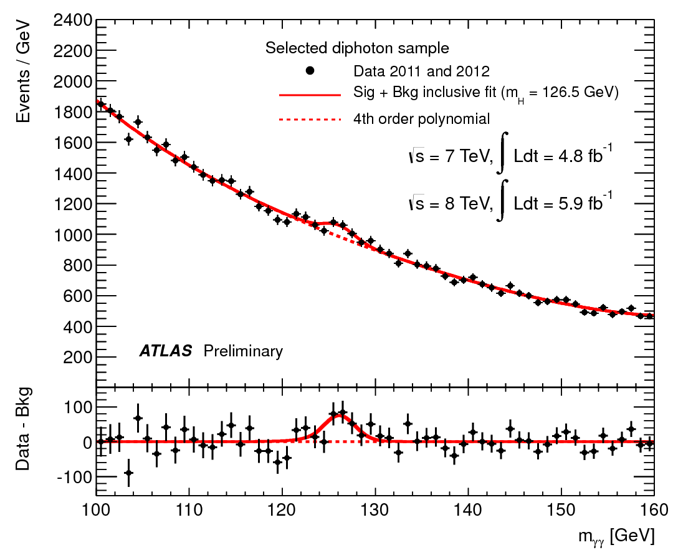
\includegraphics[width=0.4\paperwidth]{2012Higgsplot}}
	\caption{The invariant mass from pairs of photons selected in the Higgs to $\gamma\gamma$ analysis at ATLAS, as shown at the seminar at CERN on 4 July 2012. The excess of events over the background prediction around 125 GeV is consistent with predictions for the Standard Model Higgs boson.\cite{Collaboration:2627611}}
\end{figure}

\begin{figure}
	\centerline{
		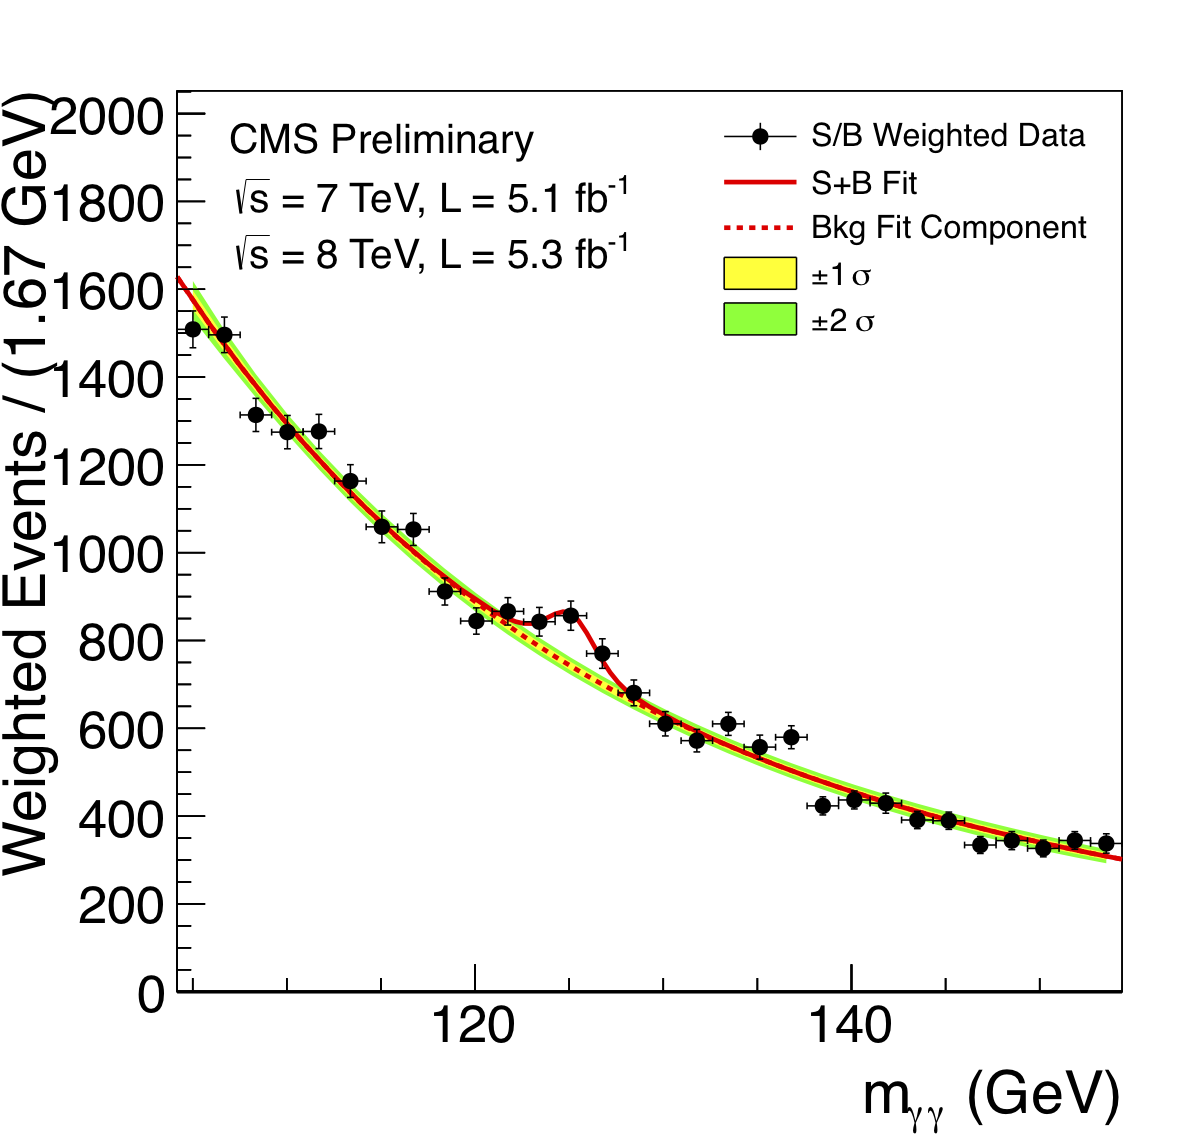
\includegraphics[width=0.4\paperwidth]{2012Higgsplot_CMS}}
	\caption{Di-photon ($\gamma\gamma$) invariant mass distribution for the CMS data of 2011 and 2012 (black points with error bars). The data are weighted by the signal to background ratio for each sub-category of events. The solid red line shows the fit result for signal plus background; the dashed red line shows only the background. \cite{Collaboration:1459463}}
\end{figure}


Usually, the background follows a pattern, for which it's possible to fit a function (in this case a fourth order polynomial).

TODO


\section{Compact Muon Solenoid}

The Compact Muon Solenoid (CMS) experiment is a general purpose particle detector, designed to observe all interactions in a collision. It's also a \textit{hermetic} detector: it blocks particles from escaping the detector undetected. Since the decay of particles can produce new particles not interacting with any part of the detector, this design allows the measurement of imbalance in momentum and energy, and these non-interacting phenomena can be inferred.

\begin{figure}
	\centerline{
		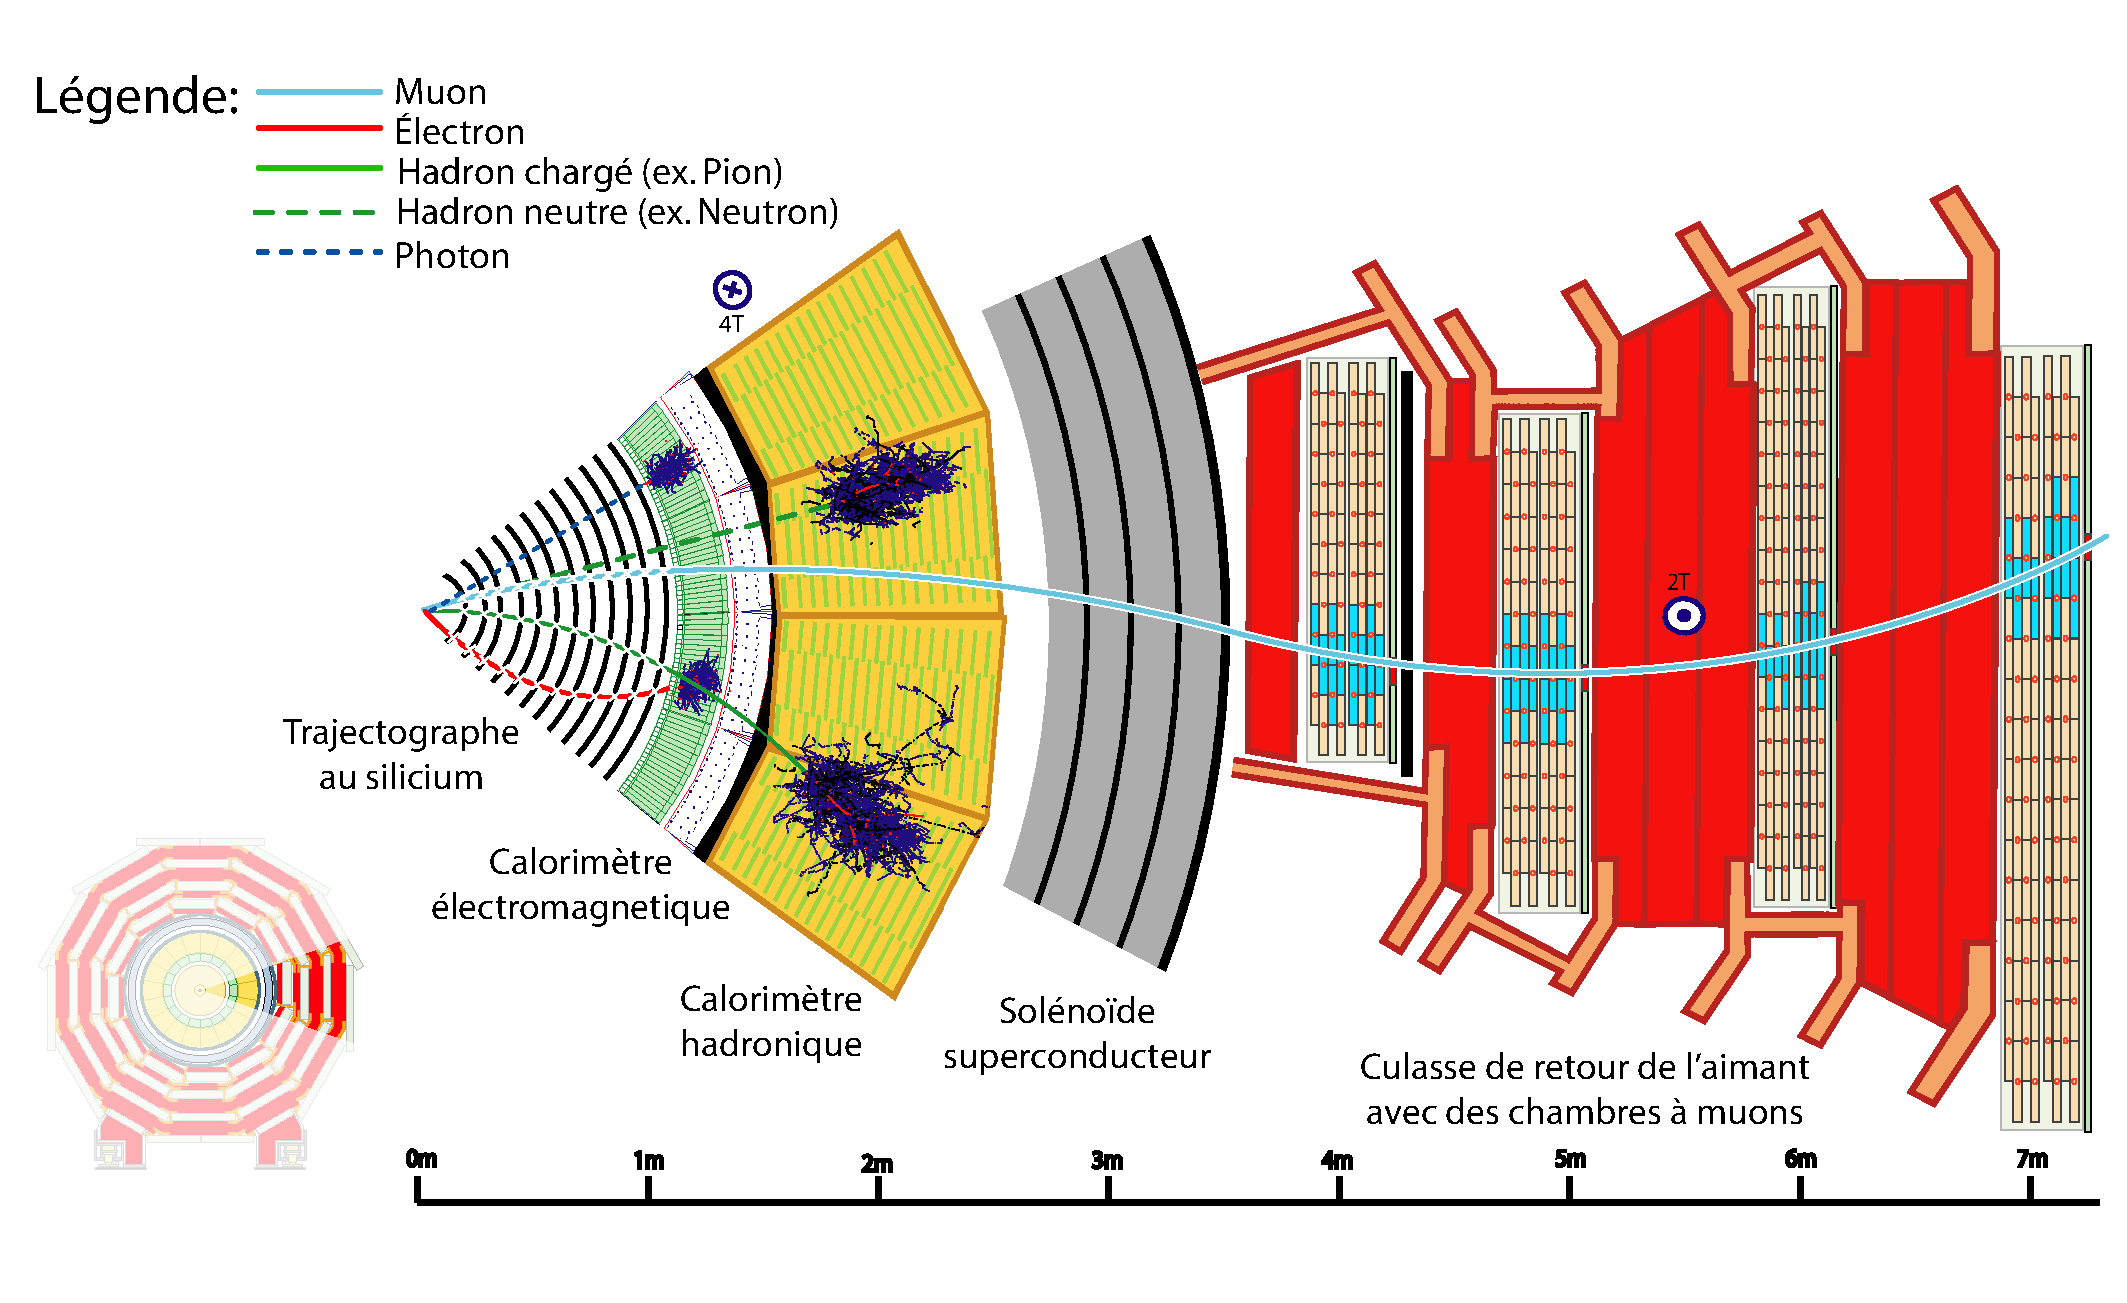
\includegraphics[width=0.75\paperwidth]{slice_white_colour_french_291016}}
	\caption{A transversal slice through the CMS detector, demonstrating the various sections of the detector
		and their designed functions. \cite{Barney:2628641}}
	\label{fig:cms2}
\end{figure}

\subsection{Silicon Tracker}

This part, the closest to the center of collision, is able to measure location, magnetic field and momentum of the particles. It can detect the decay of very short-lived particles, such as beauty quarks.

It needs to be as little as obstrusive as possibile, and it's built following the microstrip design: a large number of identical semiconductor strips laid out along one axis of a two-dimensional structure. The geometrical layout of the components allows to accurately reconstruct the track of an incoming particle of ionizing radiation.

\subsection{Electromagnetic Calorimeter}

The Electromagnetic Calorimeter (ECAL) is composed by a set of 75000 lead lungstate crystals, stopping the passing electrons and photons. When this happens, these crystals produce light as electromagnetic photon showers, measured by photodetectors.


\subsection{Hadronic Calorimeter}

The Hadronic Calorimeter (HCAL) detects hadrons and gluons with several layers of dense absoring materials and \textit{scintillators} where light pulses are produced when particles flows through.

\subsection{Superconducting Solenoid}

The Superconducting Solenoid is the largest superconducting magnet ever built. It's a huge magnet made of coils of wire that produce a uniform magnetic field when electricity flows through them. The CMS magnet is “superconducting”, allowing electricity to flow without resistance and generating a powerful magnetic field of 4 T, allowing precise momentum readings by analyzing the arcs of charged particles.

\subsection{Muon Chambers}

This section is composed of three components: Resistive Plate Chambers (RPC), Drift Tubes (DT), Cathode Strip Chambers (CSC). It relies on the strong magnetic field (\~{} 2 T, provided by the return flux outside the solenoid) to measure the curvature of the only particles that managed to reach this section: muons and neutrinos.


\begin{figure}
	\centerline{
		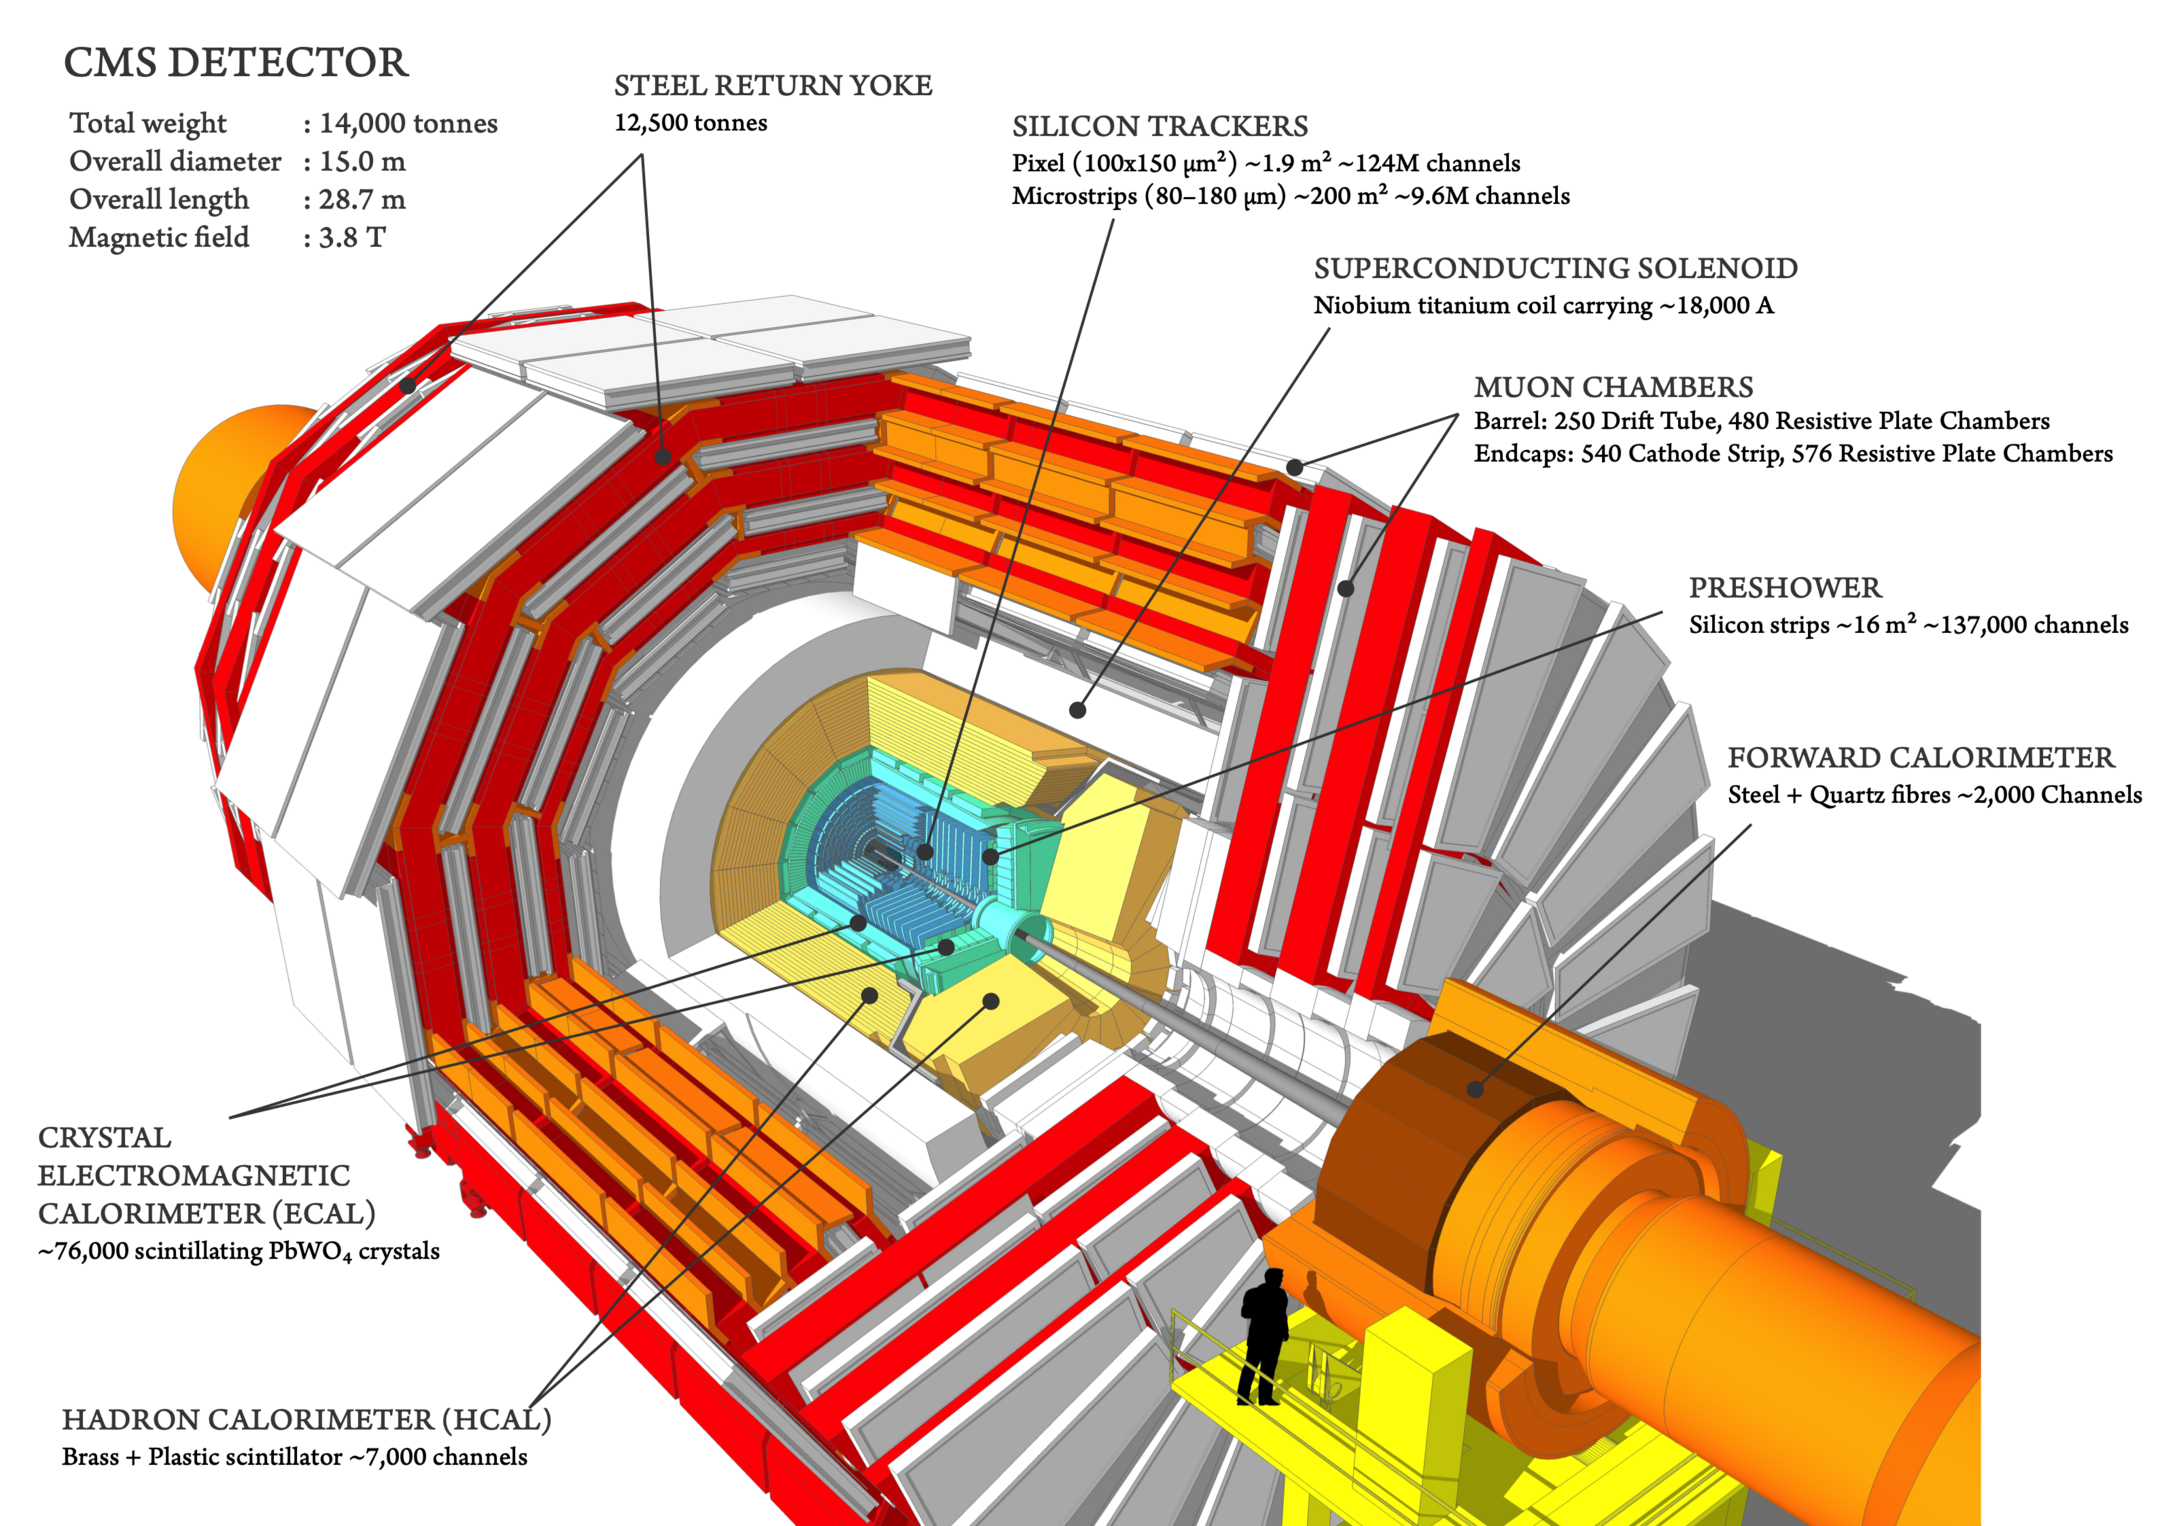
\includegraphics[width=0.8\paperwidth]{cms}}
	\caption{Cutaway diagram of the CMS detector \cite{Sakuma_2014}}
	\label{fig:cms}
\end{figure}

\section{CMS Trigger System}


The LHC generates 40 millions events per second. Each CMS event, on average, carries a payload of 1 MB of unprocessed informations. It is technologically impossible to retain this amount of data, due to hardware, software, network and storage constraints.

Furthermore, most events represent uninteresting information for the current state of physics knowledge.

The \textit{CMS Trigger System} is designed to reduce the output stream to 1000 events per second, while preserving the physics reach of the experiment.
It is composed by a hierarchical set of rules, called Trigger Nodes (or Paths): each one probes a specific patterns (physics signature) in the event or looks for specific physics objects.

This happens in two steps:

\begin{enumerate}

	\item The first level (L1) \cite{Bayatyan:706847} brings the 40 MHz to a 100 kHz rate. Here, N Trigger Algorithms are implemented on custom electronics (FPGAs and ASICs) exploiting informations from sub-detector components.

	\item A configurable set of L1 Trigger Nodes seeds Triggers in the second level (HLT), implemented in software. The event stream is further refined, selecting an average rate of 400 Hz for offline event storage and certification \cite{Khachatryan_2017}. HLT runs 600 of these independent Trigger Paths.

\end{enumerate}